
\documentclass[a4paper,11pt]{article}


%%% fontenc
%\usepackage{fontspec,xunicode,xltxtra}
%\setmainfont{Times New Roman}
%\setsansfont{Source Sans Pro}
%\setmonofont{Source Sans Pro}

%%% xeCJK
\usepackage{xeCJK}
\setCJKmainfont[BoldFont=Adobe Heiti Std]{Adobe Song Std}
\setCJKsansfont[BoldFont=Adobe Heiti Std]{Adobe Song Std}
\setCJKmonofont[BoldFont=Adobe Heiti Std]{Adobe Song Std}
\XeTeXlinebreaklocale "zh"
\XeTeXlinebreakskip=0pt plus 1pt minus 0.1pt

\usepackage{xcolor}
\usepackage{graphicx}

%%% get total page number
\usepackage{lastpage}

%%% customized definition
\makeatletter
\def\sybtitle#1{\def\@sybtitle{#1}}
\def\sybauthor#1{\def\@sybauthor{#1}}
\def\sybdate#1{\def\@sybdate{#1}}
\sybtitle{}
\sybauthor{}
\sybdate{}
\def\sybmaketitle{
  \begin{center}
  \vspace*{.8in}
  {\huge\bfseries\@sybtitle}
  \par
  \vspace{.8in}
  {\Large\@sybauthor}
  \par
  \vspace{.2in}
  \@sybdate
  \vspace{.5in}
  \end{center}
}
\makeatother
\setlength{\parindent}{0pt}
\renewcommand{\today}{\number\month 月 \number\day 日, ~\number\year 年}
\def\lt{\textless}
\def\gt{\textgreater}
\renewcommand\contentsname{\bfseries 目~~录}
\newcommand\bs{\texttt{\symbol{'134}}} % input backslash sign
%\newcommand\bs{\string\} % same as above definition
\long\def\cmd#1{\par\vspace{.5em}\hspace*{2em}#1\vspace{.5em}\par}
\def\cstr#1{\texttt{\string#1}} % e.g. \cstr{\latex}
\long\def\runcode#1{\par\bigskip#1\bigskip\par}
% 我不想看到那么多的underful hbox,尤其是minted环境加上背景色之后
\hbadness=10000
% 适当放宽overful hbox的限制,运行2pt的溢出
\hfuzz=2pt
\parskip=3\lineskip


%%% change background color & add frame for enumerate enviroment
\usepackage{mdframed}
\newmdenv[backgroundcolor=blue!10,linewidth=0pt]{coloredframe}
\newenvironment{coloredenumerate}{
  \begin{coloredframe}
  \begin{enumerate}
}{
  \end{enumerate}
  \end{coloredframe}
}

%%% geometry
\usepackage[includehead,includefoot,hmargin=21mm,vmargin=10.5mm,
            headsep=12pt,headheight=25pt]{geometry}
%\usepackage[includehead,includefoot,hmargin=1.2in,vmargin=1in]{geometry}

%%% fancyhdr
\usepackage{fancyhdr}
\makeatletter
\fancypagestyle{main} {
  \fancyhf{} % clear header & footer
  \fancyhead[L]{\bfseries\@sybtitle}
  \fancyhead[R]{\thepage/\pageref*{LastPage}}
  \renewcommand{\headrulewidth}{0.4pt} % header line
  \renewcommand{\footrulewidth}{0pt} % footer line
}
\fancypagestyle{header} {
  \fancyhf{} % clear header & footer
  \fancyfoot[C]{\roman{page}}
  \renewcommand{\headrulewidth}{0pt} % header line
  \renewcommand{\footrulewidth}{0pt} % footer line
}
\makeatother

\usepackage{titlesec}
\titleformat{\part}{\centering\Large\bfseries}{第\,\thepart\,部分}{1em}{}
\titleformat{\section}{\large\bfseries}{\thesection}{1em}{}
\titleformat{\subsection}{\normalsize\bfseries}{\thesubsection}{1em}{}
%\titlespacing*{章节命令}{左边距}{上文距}{下文距}[右边距]
\titlespacing*{\section}{0pt}{2\baselineskip}{\parsep}


\usepackage{hyperref}

%%% perfect source code display
\usepackage{minted}
%\usemintedstyle{colorful}
\definecolor{srcbg}{rgb}{0.95,0.95,0.95}
\newminted{java}{linenos,tabsize=4,bgcolor=srcbg}
\newminted{xml}{linenos,tabsize=4,bgcolor=srcbg}
\newminted{cpp}{linenos,tabsize=4,bgcolor=srcbg}
\newminted{bash}{linenos,tabsize=4,bgcolor=srcbg}
\newminted{latex}{linenos,tabsize=4,bgcolor=srcbg}



\usepackage{xcolor}
\colorlet{HEADCOLOR}{red!50}
\colorlet{BRANCHCOLOR}{blue!50}
\colorlet{WORKCOLOR}{gray!50}
\colorlet{INDEXCOLOR}{cyan!50}
\colorlet{COMMITCOLOR}{green}

\usepackage{tikz}
\usetikzlibrary{shapes,arrows,positioning,calc,backgrounds,matrix,fit,decorations.pathreplacing}
\tikzset{
  basic-style/.style = {
    rectangle, rounded corners=2pt, draw, thick,
    fill=#1,
    minimum height=15pt,
    minimum width=1.5cm,
    inner sep=1pt
  },
  commit-style/.style = {
    basic-style=COMMITCOLOR
  },
  index-style/.style = {
    basic-style=INDEXCOLOR,
    minimum width=2.5cm
  },
  work-style/.style = {
    basic-style=WORKCOLOR,
    minimum width=2.5cm
  },
  branch-style/.style = {
    basic-style=BRANCHCOLOR
  },
  head-style/.style = {
    basic-style=HEADCOLOR
  },
  cmd-style/.style = {
    #1=5pt
  },
  cmd-style/.default = right,
  main-style/.style = {
    execute at end picture = {
      \begin{pgfonlayer}{background}
        \path[fill=gray!20,rounded corners]
          ([xshift=-0.2cm,yshift=-0.2cm]current bounding box.south west) rectangle
          ([xshift=0.2cm,yshift=0.2cm]current bounding box.north east);
          %(current bounding box.south west) rectangle
          %  (current bounding box.north east);
        \end{pgfonlayer}
    }
  },
  file-style/.style = {
    draw=red, fill=yellow!30, inner sep=2pt
  },
  dir-style/.style = {
    fill=green!50,inner sep=2pt
  },
  dir-bg-style/.style = {
    fill=cyan!30,rounded corners
  },
  every edge/.style = {draw, ->, >=latex', thick}
}

%%%%% new definitions %%%%%

\newlength\commitDistance
\setlength\commitDistance{0.5cm}
\newlength\indexWorkDistance
\setlength\indexWorkDistance{2\commitDistance}

\newcommand\displayName[1]{\ttfamily\bfseries #1}
\newcommand\commandName[1]{\ttfamily\bfseries\small #1}

\def\createNode style:#1 name:#2 display:#3 direct:#4 distance:#5 to:#6;{
  \node [#1, #4=#5 of #6] (#2) {#3}
        edge [#4] (#6);
}
\def\createCommit name:#1 display:#2 direct:#3 to:#4;{
  \node [commit-style, #3=\commitDistance of #4] (#1) {#2}
        edge [#3, COMMITCOLOR] (#4);
}
\def\createBranch name:#1 display:#2 direct:#3 to:#4;{
  \node [branch-style, #3=0.75\commitDistance of #4] (#1) {#2}
        edge [#3, BRANCHCOLOR] (#4);
}
\def\createHead direct:#1 to:#2;{
  \node [head-style, #1=0cm of #2] (head) {\displayName HEAD};
}
\def\createIndex to:#1;{
  \node [index-style, below=2\commitDistance of #1] (index) {\displayName Index};
}
\def\createWork to:#1;{
  \node [work-style, below=2\commitDistance of #1] (work) {\displayName Work DIR};
}

\newcommand\makeOutline{
  %\useasboundingbox (-0.1,-3.6) rectangle (10.7,2);
  \node[right] (dumy) at (0,0) {\dots};
  \createCommit name:a display:{\displayName A} direct:right to:dumy;
  \createCommit name:b display:{\displayName B} direct:right to:a;
  \createCommit name:c display:{\displayName C} direct:right to:b;
  \createCommit name:d display:{\displayName D} direct:right to:c;
  \createCommit name:e display:{\displayName E} direct:right to:d;

  \createIndex to:c;
  \createWork to:index;
}

\newcommand\createMatrix[2]{
  \matrix [
    matrix of nodes,
    nodes={rectangle,draw=red,fill=yellow!30,minimum width=1.3cm,font=\ttfamily\small,inner sep=2pt},
    row sep=-\pgflinewidth,
    column sep=-\pgflinewidth,
  ] (m#1) at #2 {
    \textcolor{blue}{list-#1}\\
    a.h\\
    b.h\\
    c.h\\
    $d_{v#1}.h$\\
  };
}

\newcommand\createHashMatrix[2]{
  \matrix [
    matrix of nodes,
    nodes={rectangle,draw=red,fill=yellow!30,minimum width=1.3cm,font=\ttfamily\small,inner sep=2pt},
    row sep=-\pgflinewidth,
    column sep=-\pgflinewidth,
  ] (m#1) at #2 {
    \textcolor{blue}{hash-#1}\\
    a47c3\\
    b325c\\
    c10b9\\
    \textcolor{cyan}{da98#1}\\
  };
}

\usepackage{calc} % for \real control sequence
%%%%%%%%%%%%%%%%%%%%%
\newlength {\boxw}
\newlength {\boxh}
\newlength {\boxd}
\newlength {\boxroundness}
\newlength {\boxshadowsize}
\newlength {\shadowiter}
\newlength {\innersep}


\setlength {\boxshadowsize}{6pt}
\setlength {\boxroundness}{3pt}

\newsavebox {\shadowblockbox}
\newenvironment{shadowblock}[4] % {minipage width}{fill color}{draw color}{inner sep}
{\def\fillcolor{#2}\def\drawcolor{#3}%
  \setlength {\innersep}{#4}%
  \begin{lrbox}{\shadowblockbox}\begin{minipage}{#1}}
{\end{minipage}\end{lrbox}
  % draw the textbox
  \settowidth {\boxw}{\usebox{\shadowblockbox}}   % get box's width
  \settoheight {\boxh}{\usebox{\shadowblockbox}}  % get box's height
  \settodepth {\boxd}{\usebox{\shadowblockbox}}   % get box's depth

  \addtolength {\boxh}{\boxd}
  \addtolength {\boxw}{2\boxroundness}
  \addtolength {\boxh}{2\boxroundness}
  \addtolength {\boxw}{2\innersep}
  \addtolength {\boxh}{2\innersep}

  
\begin{tikzpicture}
    % draw the shadow
    \foreach \x in {0,0.05,...,1} {
      \setlength{\shadowiter}{\boxshadowsize*\real{\x}}
      \fill[xshift=\boxshadowsize-1pt,yshift=-\boxshadowsize+1pt,
          black,opacity=0.04,rounded corners=\boxroundness]
          (\shadowiter,\shadowiter) rectangle +(\boxw-2\shadowiter,\boxh-2\shadowiter);
    }
    % draw the box border
    \filldraw[fill=\fillcolor,draw=\drawcolor,rounded corners=\boxroundness]
        (0,0) rectangle (\boxw,\boxh);
    % draw the content
    \node[xshift=\boxroundness,yshift=\boxroundness,inner sep=\innersep,outer sep=0pt,anchor=south west]
        at (0,0) {\usebox{\shadowblockbox}};
  \end{tikzpicture}
}

\newcommand\gitcmd[1]{%
%\begin{center}
%  \noindent\fcolorbox{white}{yellow!20}{%
%    \begin{minipage}{.7\textwidth}
%      \centering\Large
%      \texttt{#1}
%    \end{minipage}}
%\end{center}

\begin{center}
  \begin{shadowblock}{0.9\textwidth}{yellow!50}{black!50}{0pt}
  \centering\Large
  \texttt{#1}
  \end{shadowblock}
\end{center}
}

%\newsavebox{\framedtextbox}
%\newenvironment{framedtext}[1] % minipage width
%{\begin{lrbox}{\framedtextbox}\begin{minipage}{#1}\centering}
%{\end{minipage}\end{lrbox}
%  % put box in a tikz node, and draw the node.
%  \begin{tikzpicture}
%    \node [fill=gray!20,rounded corners] at (0,0) {\usebox{\framedtextbox}};
%  \end{tikzpicture}
%}
\newenvironment{framedtext}
{\begin{center}\begin{shadowblock}{0.7\textwidth}{gray!20}{red}{10pt}\ttfamily}
{\end{shadowblock}\end{center}}

\newcommand\surrounded[1]{
  \textless#1\textgreater
}

\newcommand\optionalSurrounded[1]{
  [\textless#1\textgreater]
}


\sybtitle{Java Notes}
\sybauthor{孙延宾}
\sybdate{\today}

\begin{document}
\tt % I love Typewriter font.
%%%%%%%% the title page and toc %%%%%%%%%%
\pagestyle{header}
\sybmaketitle
\tableofcontents
\newpage

%%%%%%% the main content %%%%%%%%%
\pagestyle{main}
\setcounter{page}{1}

\part[Basic Usage]{Basic Usage}

\section[Enumeration vs Iterator]{Enumeration vs Iterator}
Enumeration和Iterator都是用于遍历集合,Enumeration主要用于遍历
Vector、HashTable,而Iterator用于遍历其他集合。两者的主要区别是:
Enumeration不可以在遍历过程中删除元素,而Iterator则可以,
比较Enumeration和Iterator的定义就可以明确这一点。

下面是Enumeration的定义,

\begin{javacode}
public interface Enumeration<E> {
  boolean hasMoreElements();
  E nextElement();
}
\end{javacode}

下面是Iterator的定义,

\begin{javacode}
public interface Iterator<E> {
  boolean hasNext();
  E next();
  void remove();
}
\end{javacode}

另附使用实例(Vector既可以Enumeration遍历也可用Iterator遍历),

\begin{javacode}
Vector<String> v = new Vector<String>();
v.add("A");
v.add("B");
v.add("C");

// 使用Enumeration遍历
// 'for' version
String elem;
for(Enumeration<String> e = v.elements(); e.hasMoreElements(); ) {
  elem = e.nextElement();
  System.out.println(elem);
}
// 'while' version
Enumeration<String> e = v.elements();
while(e.hasMoreElements()) {
  elem = e.nextElement();
  System.out.println(elem);
}

// 使用Iterator遍历
// 'for' version
String cur;
for(Iterator<String> iter = v.iterator(); iter.hasNext(); ) {
  cur = iter.next();
  System.out.println(cur);
  if("B".equals(cur)) {
    iter.remove();
  }
}
// 'while' version
Iterator<String> iter = v.iterator();
while(iter.hasNext()) {
  cur = iter.next();
  System.out.println(cur);
  if("B".equals(cur)) {
    iter.remove();
  }
}
\end{javacode}

\section[遍历Map]{遍历Map}
遍历Map时需要从collection的视角去看Map。

\begin{javacode}
public void operateMap() {
  HashMap<String, String> info = new HashMap<String, String>() {
    private static final long serialVersionUID = 1L;
    {
      put("John", "42");
      put("Eric", "43");
      put("Waston", "44");
    }
  };

  /*
   * Collection<E> interface extends Iterable<T> interface,
   * so all Collection including Set<E>, List<E>, Queue<E>
   * can get an Iterator via iterator() method.
   */

  // 遍历Map - 1
  Iterator<Entry<String, String>> entryIter = info.entrySet().iterator();
  while(entryIter.hasNext()) {
    Entry<String, String> entry = entryIter.next();
    System.out.println("key: " + entry.getKey() + ", value: " + entry.getValue());
  }

  // 遍历Map - 2
  Iterator<String> keyIter = info.keySet().iterator();
  while(keyIter.hasNext()) {
    String key = keyIter.next();
    String value = info.get(key);
    System.out.println("key: " + key + ", value: " + value);
  }

  // 遍历Map - 3,遍历Value
  Iterator<String> valueIter = info.values().iterator();
  while(valueIter.hasNext()) {
    String value = valueIter.next();
    System.out.println("value: " + value);
  }
}
\end{javacode}

\section[Inner Class]{Inner Class}
Java中,Inner class的field/method相当于Outer class的field/method,
只不过要通过Inner class或Inner class的对象对其进行访问而已。

\subsection[内部类的可见性]{内部类的可见性}
内部类的field/method跟外部类的field/method本质上是一样的,只是访问
方式不同而已,所以内部类和外部类相互之间是“完全透明”的。

\subsection[Create object of Inner class ]{Create object of Inner class}
由于non-static inner class依附于outer class而存在,所以创建这种类型的
对象时必须有outer class对象存在才行;而对于static inner class则无此限制。

\begin{javacode}
class Outer {
  private int out = 42;

  // non-static inner class
  public class InstanceInner {
    private int instanceInner = out;
  }

  // static inner class
  public static class StaticInner {
    private static int staticInner;
  }

  private void out() {
    // access 'private' field of inner class
    int i = new InstanceInner().instanceInner;
    int k = StaticInner.staticInner;
  }
}

class Test {
  void test() {
    Outer outer = new Outer();
    // non-static内部类依附于外部类而存在,所以实例化时必须存在外部类对象
    InstanceInner iInner = outer.new InstanceInner();
    // static内部类则可直接实例化,不需外部类对象存在
    StaticInner sInner = new Outer.StaticInner();
  }
}
\end{javacode}

\subsection[Inner class for JVM]{Inner class for JVM}
在JVM看来,inner class是如何表示的呢?

\emph{在JVM中,根本没有inner class这个概念!一切都是顶级类!}

只是内部类最终编译成class文件时,其名称是...\$...class这样的形式。

啊?那岂不是说:类的private成员可以被外部类(not outer class)访问?

是的,只不过这里的情形比较特殊,看下面的代码,

\begin{javacode}
class OuterClass {
  private int out = new InnerClass().in;
  class InnerClass {
    private int in = 0;
  }
}
\end{javacode}

分别反编译OuterClass.class和OuterClass\$InnerClass.class,
在OuterClass.class中可以看到这样的代码:

\begin{javacode}
13: invokestatic #17; //Method com/example/javademo/OuterClass$InnerClass
                  .access$0:(Lcom/example/javademo/OuterClass$InnerClass;)I
16: putfield #21; //Field out:I
\end{javacode}

这便是new InnerClass().in编译之后的代码。再看OuterClass\$InnerClass.class
的反编译结果:

\begin{javacode}
static int access$0(com.example.javademo.OuterClass$InnerClass);
  Code:
    Stack=1, Locals=1, Args_size=1
    0: aload_0
    1: getfield #17; //Field in:I
    4: ireturn
\end{javacode}

这个静态函数其实只是把属性"in"的值返回而已,这个静态函数叫做sythetic函数,
也叫做bridge函数。进一步查看.class的二进制数据(用十六进制编辑器),可以看到
该函数的access\_flag设置为10 08,即ACC\_SYNTHETIC | ACC\_STATIC。

\section[Double braces initialization]{Double braces initialization}
要讲明白双大括号初始化就要先了解什么是instance initializer和static initializer,
该部分Java语言规范在\href{http://docs.oracle.com/javase/specs/jls/se7/html/jls-8.html#jls-8.6}{JLS 8.6}。

\begin{javacode}
class Initializer {

  // executed when an instance of the class is created
  static {
    System.out.println("static initializer");
  }

  // executed when the class is initialized
  {
    System.out.println("instance initializer");
  }

  public Initializer() {
    System.out.println("constructor");
  }

  void initialize() {
    System.out.println("instance method");
  }
}
\end{javacode}

执行顺序:static initializer, instance initializer, constructor。

Java支持匿名内部类(Inner anonymous class),既然是匿名的,就无法在其他地方引用,
因此也就只能在创建类的同时创建对象(毕竟,类不用来创建对象还能干啥呢),内层的
大括号即为instance initializer。

于是乎,有了下面的代码,

\begin{javacode}
package com.example.javademo;
Class DoubleBraceTest {
  void test() {
    // 初始化HashMap
    HashMap<String, String> hm = new HashMap<String, String>() {
      // instance initializer(对比static initializer)
      {
        // 匿名内部类的this指向父类(即HashMap)对象
        this.put("k1", "v1");
        this.put("k2", "v2");
        this.put("k3", "v3");
      }
    }

    // 任意类都可以,Base是任意自定义类
    Base b = new Base() {
      {
        setName(Inner anonymous class, instance initializer.);
      }
    }

    // result: super class: java.util.HashMap
    System.out.println("super class: " + hm.getClass().getSuperclass().getName());
    // result: class name: com.example.javademo.DoubleBraceTest$2
    System.out.println("class name: " + hm.getClass().getName());
  }
}
\end{javacode}

注意:double braces initialization是不鼓励使用的,因为它本质上是定义了一个
匿名内部类,因此实例化的instance会一直保存对外部类(DoubleBraceTest类)实例
的引用,并且这也会让类加载器管理更多的类。

\section[Polymorphism - 多态]{Polymorphism - 多态}
在Java中(其他OOP中也是如此),Polymorphism(多态)是一个概念,它用于method的定义,
有两种表现形式:override和overload。两种多态形式各有不同的限定条件。

\subsection[override]{override}
父类方法和子类方法构成override必须满足如下条件:

\begin{enumerate}
  \item 子类方法和父类方法的name、parameters、return type必须完全一样
  \item 子类方法不能缩小(reduce)父类方法的访问权限
  \item 子类方法不能扩大或者改变父类方法的异常范围,详见第\ref{sec:exceptions-in-override}节
\end{enumerate}

注意:final修饰的方法不能被override。

\subsection[overload]{overload}
位于同一个类中或者分别位于父类和子类中的两个方法,构成overload必须满足如下条件:

\begin{enumerate}
  \item parameters(包括参数类型、个数、顺序)不能完全相同
\end{enumerate}

注意,如果两个方法参数完全相同而只是返回值不同,则它们不构成overload关系。

\section[静态方法能否被override]{静态方法能否被override}
静态方法(类方法)能否被覆盖(override)?

这个问题本身就是错误的!

override被设计用于instance methods,而不是用于static methods。
类加载之后,static method放置在Method Area,因此每个类,不论子类父类,都有自己
单独的static field和static method,相互之间没有任何关系。

\begin{javacode}
class Base {
  public static void staticPrint() {
    System.out.println("Base static method");
  }
  public void instancePrint() {
    System.out.println("Base instance method");
  }
}

class Derived extends Base {
  public static void staticPrint() {
    System.out.println("Derived static method");
  }
  @Override
  public void instancePrint() {
    System.out.println("Derived instance method");
  }
}

Base base = new Derived();
// result: Base static method
base.staticPrint();
// result: Derived nstance method
base.instancePrint();
// result: Derived static method
((Derived) base).staticPrint();
\end{javacode}

需要注意的是:static method是静态绑定的,即在编译期就绑定完毕,
因此base.staticPrint()会被绑定到Base类的static method;
而instance method是动态绑定的,即在运行期才会寻找instance数据
(位于Heap中,base的instance数据根据Derived类实例化),
查找method的bytecode然后绑定。

\section[Exceptions in Java]{Exceptions in Java}
Java中的异常分为两类:checked exception和runtime exception(uncheck exception),
如图\ref{fig:exceptions}所示,
RuntimeException及其子类叫做runtime exception,也叫做uncheck exception,
Exception的其他子类叫做checked exception。

\begin{figure}
  \centering
  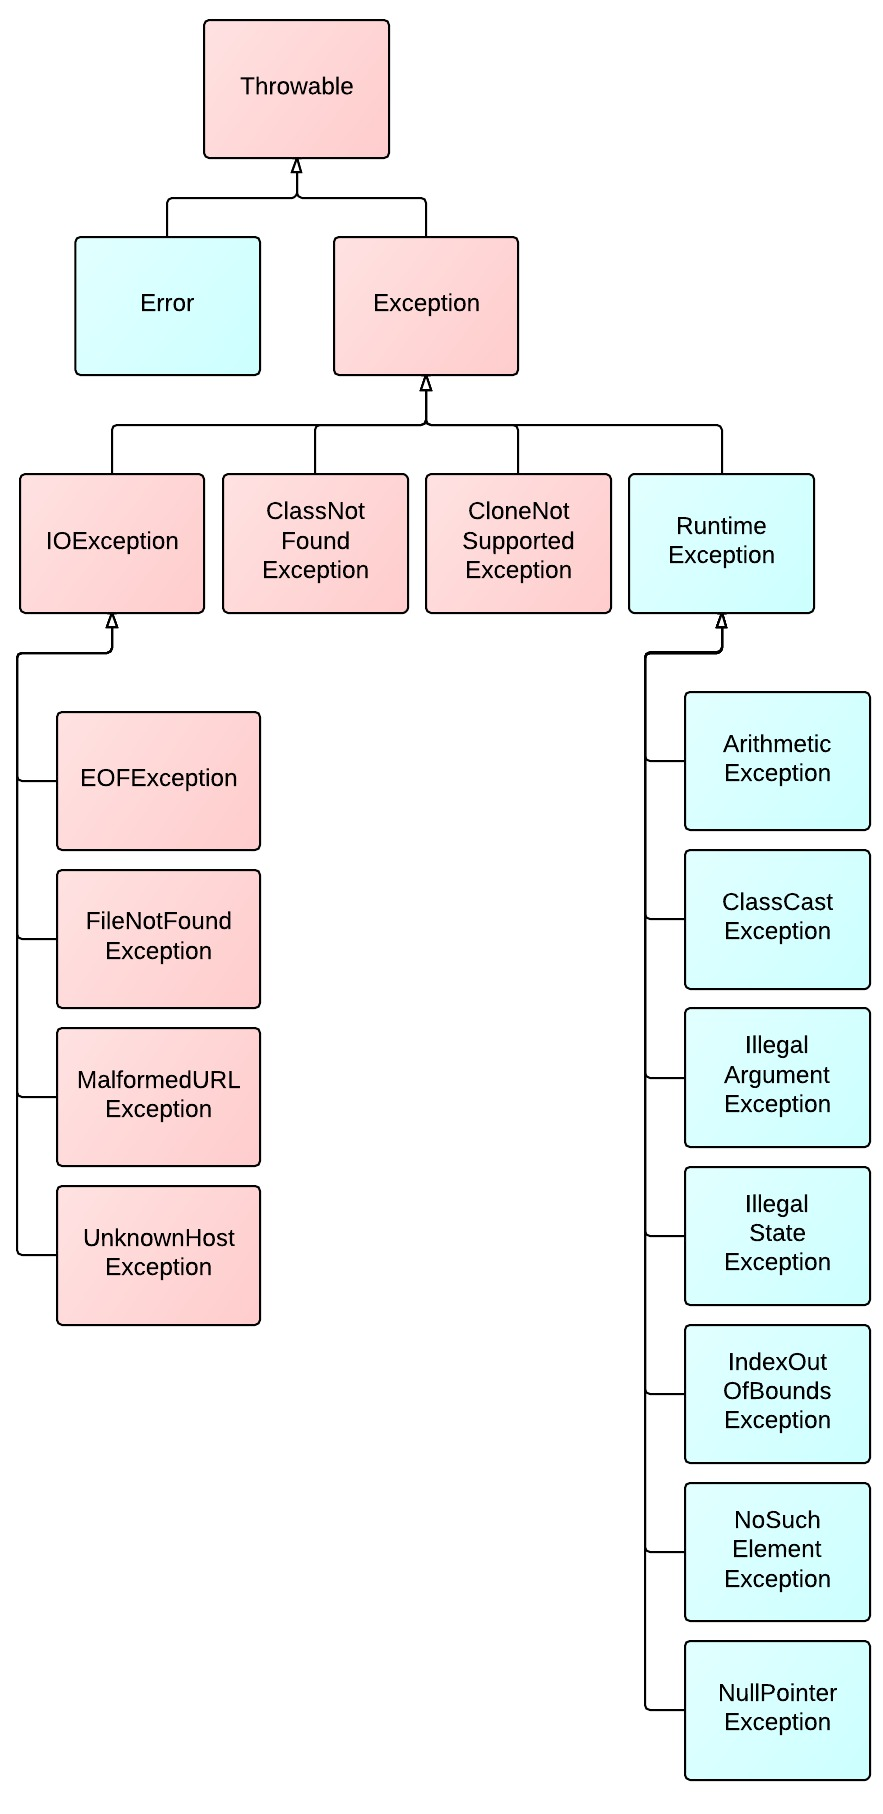
\includegraphics[width=0.7\textwidth]{picturedir/JavaExceptions.jpeg}\\
  \caption{Java的异常体系}\label{fig:exceptions}
\end{figure}

\subsection[名字的由来]{名字的由来}
所谓的checked与uncheck指的是compiler的行为,即compiler在编译时(废话,肯定是编译时)
作检查(check)的exception叫做checked exception,其他exception叫做runtime exception,
也叫做uncheck exception,

\begin{javacode}
class ExceptionTest {
  void testCheckedException() throws IOException { }
  void testRuntimeException() throws IndexOutOfBoundsException { }
  void test() {
    testCheckedException(); // compile error
    testRuntimeException(); // no compile error
  }
}
\end{javacode}

\subsection[设计的初衷]{设计的初衷}
在一个方法的实现者角度来看,checked exception意味着我知道在该方法被调用的过程中
可能会发生某些异常,但是对此我无能为力,我只能throws exception(方法签名中)以提醒你,
作为方法调用者,你要自己catch这些异常。比如某个文件正在读取时被其他进程删除了,
又比如正在进行网络数据传输却突然断网了。这些异常是callee用来提醒caller的,compiler
会检查这些异常,提醒caller进行异常捕获。

其他所有的exception都是runtime exception,如NullPointerException,它意在曝露出
方法实现上的错误,如果有,这样的exception越早曝露越好,此时我们必须修改代码来除错。

从两种异常的设计初衷来看,作为方法的调用者(callee),应该捕获所有checked exception
(废话,不捕获就无法通过编译啊)并作相应处理,如给用户友好的错误提示;而runtime exception
则不应该捕获。

\section[override方法中的exception]{override方法中的exception}
\label{sec:exceptions-in-override}
在子类方法和父类方法进行override时,对子类方法和父类方法所抛出的异常有如下要求:

\begin{enumerate}
  \item 不论父类方法抛出何种异常,子类方法都可以不抛出任何异常
  \item 父类方法和子类方法所抛出的任何runtime异常都不受限制
  \item 子类方法抛出的checked异常必须equal或者derive父类方法抛出的checked异常
\end{enumerate}

\begin{javacode}
class Base {
  public void foo() throws IOException { }
  public void bar() throws IOException { }
  public void base1() throws IOException { }
  public void base2() throws ArithmeticException { }
  public void base3() throws IOException { }
  public void base4() throws ArithmeticException { }
  public void base5() { }
}

class Derived extends Base {
  @Override
  public void foo() throws FileNotFoundException { } // allowed
  @Override
  public void bar() throws SQLException { } // NOT allowed

  @Override
  public void base1() { } // allowed, do not throw any exception
  @Override
  public void base2() throws IndexOutOfBoundsException { } // allowed
  @Override
  public void base3() throws IndexOutOfBoundsException { } // allowed
  @Override
  public void base4() throws IOException { } // NOT allowed
  @Override
  public void base5() throws IOException { } // NOT allowed
}
\end{javacode}

IOException、FileNotFoundException、SQLException都是checked异常,并且
FileNotFound\-Exception是IOException的子类,ArithmeticException和
IndexOutOfBoundsException都是runtime异常。注意,base4(), base5()两种
情况是不允许的!

\emph{为何要作此限制呢?}

考虑如下情形,

\begin{javacode}
Base base = new Derived();
try {
  base.bar();
} catch(??? e) {
  // 这里应该捕获何种异常类型呢?
}
try {
  base.foo();
} catch(IOException e) {
  // 这里应该捕获的异常类型就很明确了!
}
\end{javacode}


\section[关于this和super]{关于this和super}
this和super两个关键字值得研究,他们有本质的区别。

\emph{this、super是对象的两个属性},这种说法是及其错误的!\\
\emph{父类对象}这一说法也是及其错误的!没有这样的对象!

\subsection[this]{this}
this并非instance的field,this其实压根儿就不在heap中,this(的值)存在于thread stack中的
frame中的Local Variable的index 0处,它是JVM自动生成的。

\subsection[super]{super}
super就更让人大跌眼镜了,super不仅不是instance的field,它其实压根儿“不存在”,super
在compile时被翻译为this(它们的值相等),当然如果子类中field、method有隐藏父类field、method的
情况时,compiler也在此时一并处理了。这不仅让我想起来Clojure里的Reader Macro...

\subsection[没有父类对象]{没有父类对象}
加载子类时,父类当然是要一并加载的,但是创建子类对象时并不会创建父类对象,而是将
父类对象的fields一并存储到子类对象中(父类的method存在于Method Area中),并且这些
属性排列还有一定规则:先排放父类属性,再排放子类属性!

\subsection[Example]{实例}
看下面的代码,

\begin{javacode}
void test() {
  int result;

  this.print();
  super.print();

  result = this.testField;
  result = super.testField;
}
\end{javacode}

下面是对应的bytecode,
\begin{verbatim}
0:   aload_0
1:   invokevirtual   #34; //Method print:()V
4:   aload_0
5:   invokespecial   #36; //Method com/example/javademo/A.print:()V
8:   aload_0
9:   getfield        #12; //Field testField:I
12:  istore_1
13:  aload_0
14:  getfield        #37; //Field com/example/javademo/A.testField:I
17:  istore_1
18:  return
\end{verbatim}

下面是对应的Local Variables,
\begin{verbatim}
LocalVariableTable:
  Start   Length  Slot  Name    Signature
  0       19      0     this    Lcom/example/javademo/B;
  13      6       1     result  I
\end{verbatim}

可见,无论是this还是super均执行统一个对象(in heap),只是
super的方法和属性是全限定名称,以此与this的同名方法和属性
进行区分。


\part[Java IO]{Java IO}
Java的IO库位于java.io.*包中。

\section[Java file path]{Java中的文件路径}
文件路径分为相对路径和绝对路径,其中绝对路径并不唯一,如下几个路径,
\begin{itemize}
  \item C:/temp.txt
  \item C:/WINDOWS/../temp.txt
  \item C:/./././temp.txt
\end{itemize}
他们都是绝对路径,而且他们都表示同一个文件,于是就产生一个问题,
对于任意一个文件,有没有一个“标准”的绝对路径呢?有,而且不同操作系统
有不同的规定,这个标准的绝对路径就叫做cannonical path,可见
cannonical path也是一个绝对路径,只是它是一个特殊的绝对路径而已。

在Java中,

\begin{javacode}
public void filePath(String path) throws IOException {
  File f = new File(path);
  System.out.println("getPath(): " + f.getPath());
  System.out.println("getAbsolutePath(): " + f.getAbsolutePath());
  System.out.println("getCannonicalPath(): " + f.getCanonicalPath());
}
// 函数调用示例
new JavaDemo().filePath("C:/./././temp.txt");
// 输出结果
// getPath(): .\.\.\temp.txt
// getAbsolutePath(): D:\eclipse\workspace-adt\JavaDemo\.\.\.\temp.txt
// getCannonicalPath(): D:\eclipse\workspace-adt\JavaDemo\temp.txt
\end{javacode}

\section[面向字节的IO接口]{面向字节的IO接口}
InputStream和OutputStream是面向字节的IO接口,它们处理的是字节流

\subsection[InputStream]{InputStream}
\begin{figure}
  \centering
  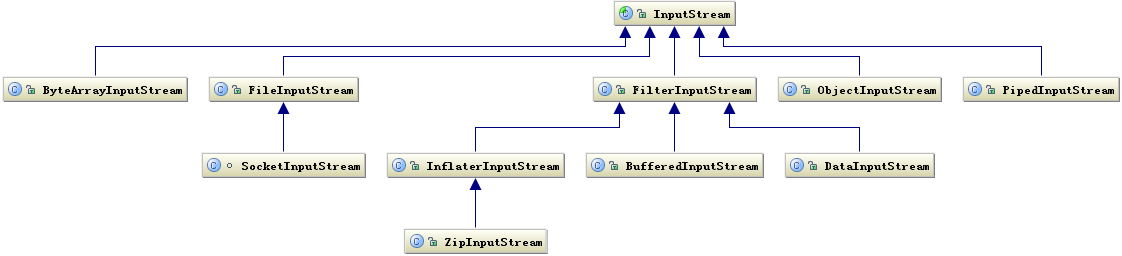
\includegraphics[width=.9\textwidth]{picturedir/inputstream.png}
  \caption{面向字节的InputStream接口}
  \label{fig:inputstream}
\end{figure}

图\ref{fig:inputstream}展示了InputStream的基本接口。
InputStream是一个抽象类,真正使用时都是使用其子类进行实例化。

\subsubsection[FileInputStream]{FileInputStream}
\subsubsection[ByteArrayInputStream]{ByteArrayInputStream}
\subsubsection[ObjectInputStream]{ObjectInputStream}
\subsubsection[PipedInputStream]{PipedInputStream}
\subsubsection[FilterInputStream]{FilterInputStream}

\subsection[OutputStream]{OuttputStream}
\begin{figure}
  \centering
  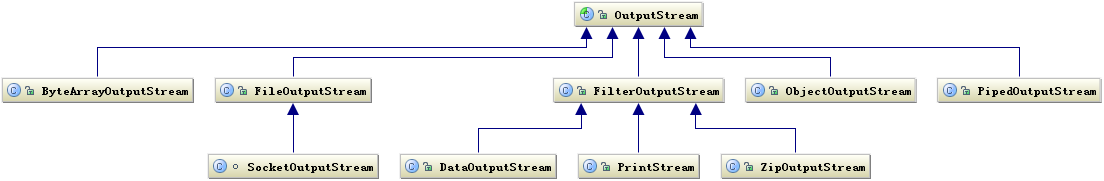
\includegraphics[width=.9\textwidth]{picturedir/outputstream.png}
  \caption{面向字节的OutputStream接口}
  \label{fig:outputstream}
\end{figure}

图\ref{fig:outputstream}展示了OutputStream的基本接口。
OutputStream是一个抽象类,真正使用时都是使用其子类进行实例化。
\subsubsection[FileOutputStream]{FileOutputStream}
\subsubsection[ByteArrayOutputStream]{ByteArrayOutputStream}
\subsubsection[ObjectOutputStream]{ObjectOutputStream}
\subsubsection[PipedOutputStream]{PipedOutputStream}
\subsubsection[FilterOutputStream]{FilterOutputStream}


\section[面向字符的IO接口]{面向字符的IO接口}
\subsection[面向字符的Input接口]{面向字符的Input接口}
\begin{figure}
  \centering
  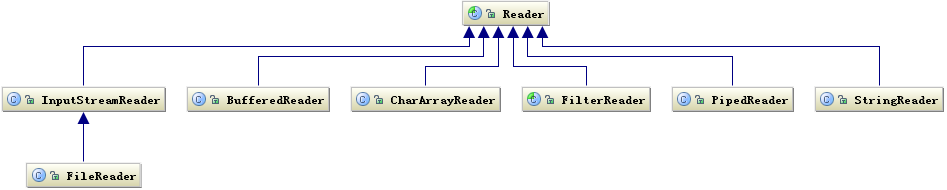
\includegraphics[width=.9\textwidth]{picturedir/reader.png}
  \caption{面向字符的Reader接口}
  \label{fig:reader}
\end{figure}

图\ref{fig:reader}展示了Reader的基本接口。

\subsection[面向字符的Output接口]{面向字符的Output接口}
\begin{figure}
  \centering
  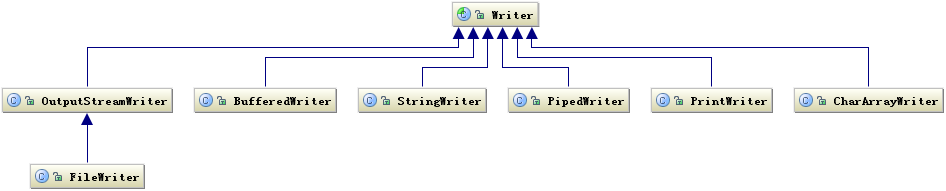
\includegraphics[width=.9\textwidth]{picturedir/writer.png}
  \caption{面向字符的Writer接口}
  \label{fig:writer}
\end{figure}

图\ref{fig:writer}展示了Writer的基本接口。



\part[Java NIO]{Java NIO}


\part[Multi-thread and Concurrency]{Multi-thread Concurrency}
\section[How to create Java thread]{How to create Java thread}

\section[package: concurrency]{package concurrency}

\section[keyword: join]{keyword: join}
join用于等待其他线程结束,如otherThread.join(),当前线程将会等待
otherThread结束后才会退出。

实例:

\begin{javacode}
public class JoinTest {
  public static void main(String[] args) {
    Thread t1 = new Thread(new MyRunnable(), "Thread-1");
    Thread t2 = new Thread(new MyRunnable(), "Thread-2");

    t1.start();
    t2.start();
    System.out.println("Main thread end.");
  }
}

class MyRunnable implements Runnable {
  String name = Thread.currentThread().getName();
  @Override
  public void run() {
    System.out.println("wtf: " + name);
    try {
      Thread.sleep(3000);
    } catch (InterruptedException e) {
      e.printStackTrace();
    }
    System.out.println(">>> " + Thread.currentThread().getName());
  }
}
\end{javacode}

注意:wtf那一行输出的是“main”,即name变量保有的是主线程的名字,WTF!

可能的输出,

\begin{bashcode}
Main thread end.
wtf: main
wtf: main
>>> Thread-1
>>> Thread-2
\end{bashcode}

\section[keyword: synchronized]{keyword: synchronized}
'synchronized'关键字用于锁住资源,从而保证多线程环境下,同一时刻只有一个
线程能拥有锁住的资源,资源用完之后释放锁。

有两种synchronized方式:
\begin{enumerate}
\item synchronized block: 只锁住该block里的资源
\item synchronized method: 锁住整个对象;如果是static方法,就锁住该Class
\end{enumerate}
另外还需注意:
\begin{itemize}
\item synchronized关键字“不能”用于构造函数和变量
\item synchronized影响效率,在真正必须的时候才使用
\item synchronized只在同一个JVM实例上有效
\item synchronized不要用于non-private的对象,以及有getter函数的private对象
\item synchronized不要用于常量池中的对象,如String对象
\end{itemize}
推荐使用方法:\\
\begin{javacode}
// dummy object variable for synchronization
private Object mutex = new Object();
int count = 0;
synchronized(mutex) {
    count++;
}
\end{javacode}

注意:synchronized需要程序员自觉才行,如果在某个线程程序员没有
使用synchronized而是直接就count++,此时synchronized就被人为的绕过
去了,尤其是用继承Thread类的方法创建线程时,这种情况更容易发生。

不要这样用:\\
\begin{javacode}
public class MyObject {
    // will lock on the object's monitor
    public synchronized void doSomething() { /* do something...*/ }

    MyObject myObject = new Myobject();
    synchronized(myObject) {
        while(true) {
            Thread.sleep(Integer.MAX_VALUE);
        }
    }
}
\end{javacode}

两个synchronized锁住的是同一个monitor,所以一旦第二个执行,
doSomething()将不可能再执行,导致死锁和DoS(Denial of Service)。

不要这样用:\\
\begin{javacode}
public class MyObject {
    public Object lock = new Object();
    public void doSomething() {
        synchronized(lock) {
            // do something...
        }
    }
}

MyObject myObject = new MyObject();
// 修改lock的引用,doSomething()函数有可能并发执行,
// 同理,有getter函数的private lock也是一样的
myObject.lock = new Object();
\end{javacode}



\section[keyword: wait, notify and notifyAll]{keyword: wait, notify and notifyAll}
wait, notify, notifyAll三个函数用于多线程竞争某个资源的情况,这三个函数在调用
之前都必须先取得“竞态资源”的monitor才行,所以这三个函数必须放到sychronized中
才行。

下面是一个生产者、消费者的实例。

测试用例:

\begin{javacode}
public class WaitNotifyTest {
  public static void main(String[] args) {
    Message msg = new Message("Init Message");
    new Thread(new Waiter(msg), "waiter1").start();
    new Thread(new Waiter(msg), "waiter2").start();

    new Thread(new Notifier(msg), "notifier").start();
    System.out.println("Main thread end.");
  }
}
\end{javacode}

竟态资源:

\begin{javacode}
class Message {
  private String msg;

  public Message(String str) {
    this.msg = str;
  }
  public String getMsg() {
    return msg;
  }
  public void setMsg(String str) {
    this.msg = str;
  }
}
\end{javacode}

消费者:

\begin{javacode}
class Waiter implements Runnable {
  private Message msg;

  public Waiter(Message m) {
    this.msg = m;
  }
  @Override
  public void run() {
    String name = Thread.currentThread().getName();
    synchronized (msg) {
      try {
        System.out.println("*" + name + "*" + " waiting msg at: "
                           + System.currentTimeMillis());
        msg.wait();
      } catch (InterruptedException e) {
        e.printStackTrace();
      }
      System.out.println("*" + name + "*" + " got msg at: "
                         + System.currentTimeMillis());
      // process the message now
      System.out.println("*" + name + "*" + " process msg: " + msg.getMsg());
    }
  }
}
\end{javacode}

生产者:

\begin{javacode}
class Notifier implements Runnable {
  private Message msg;

  public Notifier(Message msg) {
    this.msg = msg;
  }
  @Override
  public void run() {
    String name = Thread.currentThread().getName();
    System.out.println("*" + name + "*" + " started.");
    try {
      Thread.sleep(1000);
      synchronized (msg) {
        msg.setMsg("\"This is " + "*" + name + "*'s" + " msg.\"");
        //msg.notify();
        msg.notifyAll();
      }
    } catch (InterruptedException e) {
      e.printStackTrace();
    }
  }
}
\end{javacode}

注意,notifyAll会把所有等待的线程都唤醒,但是无法确定这些线程
的执行顺序,每次只能执行一个,而notify函数只能唤醒一个,随机的
一个。

执行顺序是这样的:

线程A获得msg.lock之后进入synchronized block,调用msg.wait()
阻塞A线程,然后释放msg.lock(并未退出wait()方法,在synchronized中,
没有lock就寸步难行)。线程B获得msg.lock之后进入synchronized block,
调用msg.notify()/msg.notifyAll(),通知线程A或者其他等待msg.lock
的线程,等待线程被唤醒,但是没有msg.lock仍然无法运行,之后线程B
继续执行synchronized block剩余的内容,执行完之后释放msg.lock,
正在等待的线程(如线程A)会取得msg.lock然后完成wait()方法,进而
完成synchronized block的剩余内容,之后释放msg.lock。如果线程B
调用的是msg.notifyAll()并且还有其他等待线程的话,其他等待线程中的
一个会获得msg.lock,然后执行完msg.wait()方法继而完成
synchronized block之后释放msg.lock,依次重复,直到所有等待线程
都完成这个过程,整个同步过程也就结束了。

\section[Java Memory Model]{Java Memory Model}
Java Memory Model(JMM),即Java内存模型,是存在于Java语言层面的内容,
并不涉及到JVM,JMM是用于Java线程间通讯的一套规则,目的是防止线程间
出现数据竞争。所谓的数据竞争指的是:如果A操作、B操作同时需要某些数据,
并且A、B之间存在影响(单向或者相互影响),但是并没有任何手段可以
保证它们之间的执行顺序,那么就说A、B之间存在数据竞争。如A读取某个值
而B写入某个值,但是没有任何手段可以保证它们之间的顺序,那么它们存在
数据竞争。

为此JSR-133制定了一套规则叫做happens-before规则,以此避免数据竞争。
但是需要注意的是happens-before并不仅仅是指的操作顺序,它更主要的是
明确“可见性”,如其中有一条规则如下:

\emph{对同一个monitor的unlock必须发生在其他线程lock之前}

这个很好理解,先释放锁再获取锁,但是这里不仅仅指的是操作顺序,它还要
保证,unlock之前的monitor监视的操作结果(如synchronize block里的操作)
必须能够被lock之后的线程看到,也就是说
如果Action A happens-before Action B,那么A的操作结果必须对B是
可见的,也就是说A的操作结果要写入主内存,而B在操作之前必须先从主内存
中同步数据到它的工作内存(e.g. CPU Cache)。


\part[JVM]{Java Virtual Machine}
JVM Internal Architecture, see figure \ref{fig:jvm} and \ref{fig:jvm2}.
\begin{figure}
  \centering
  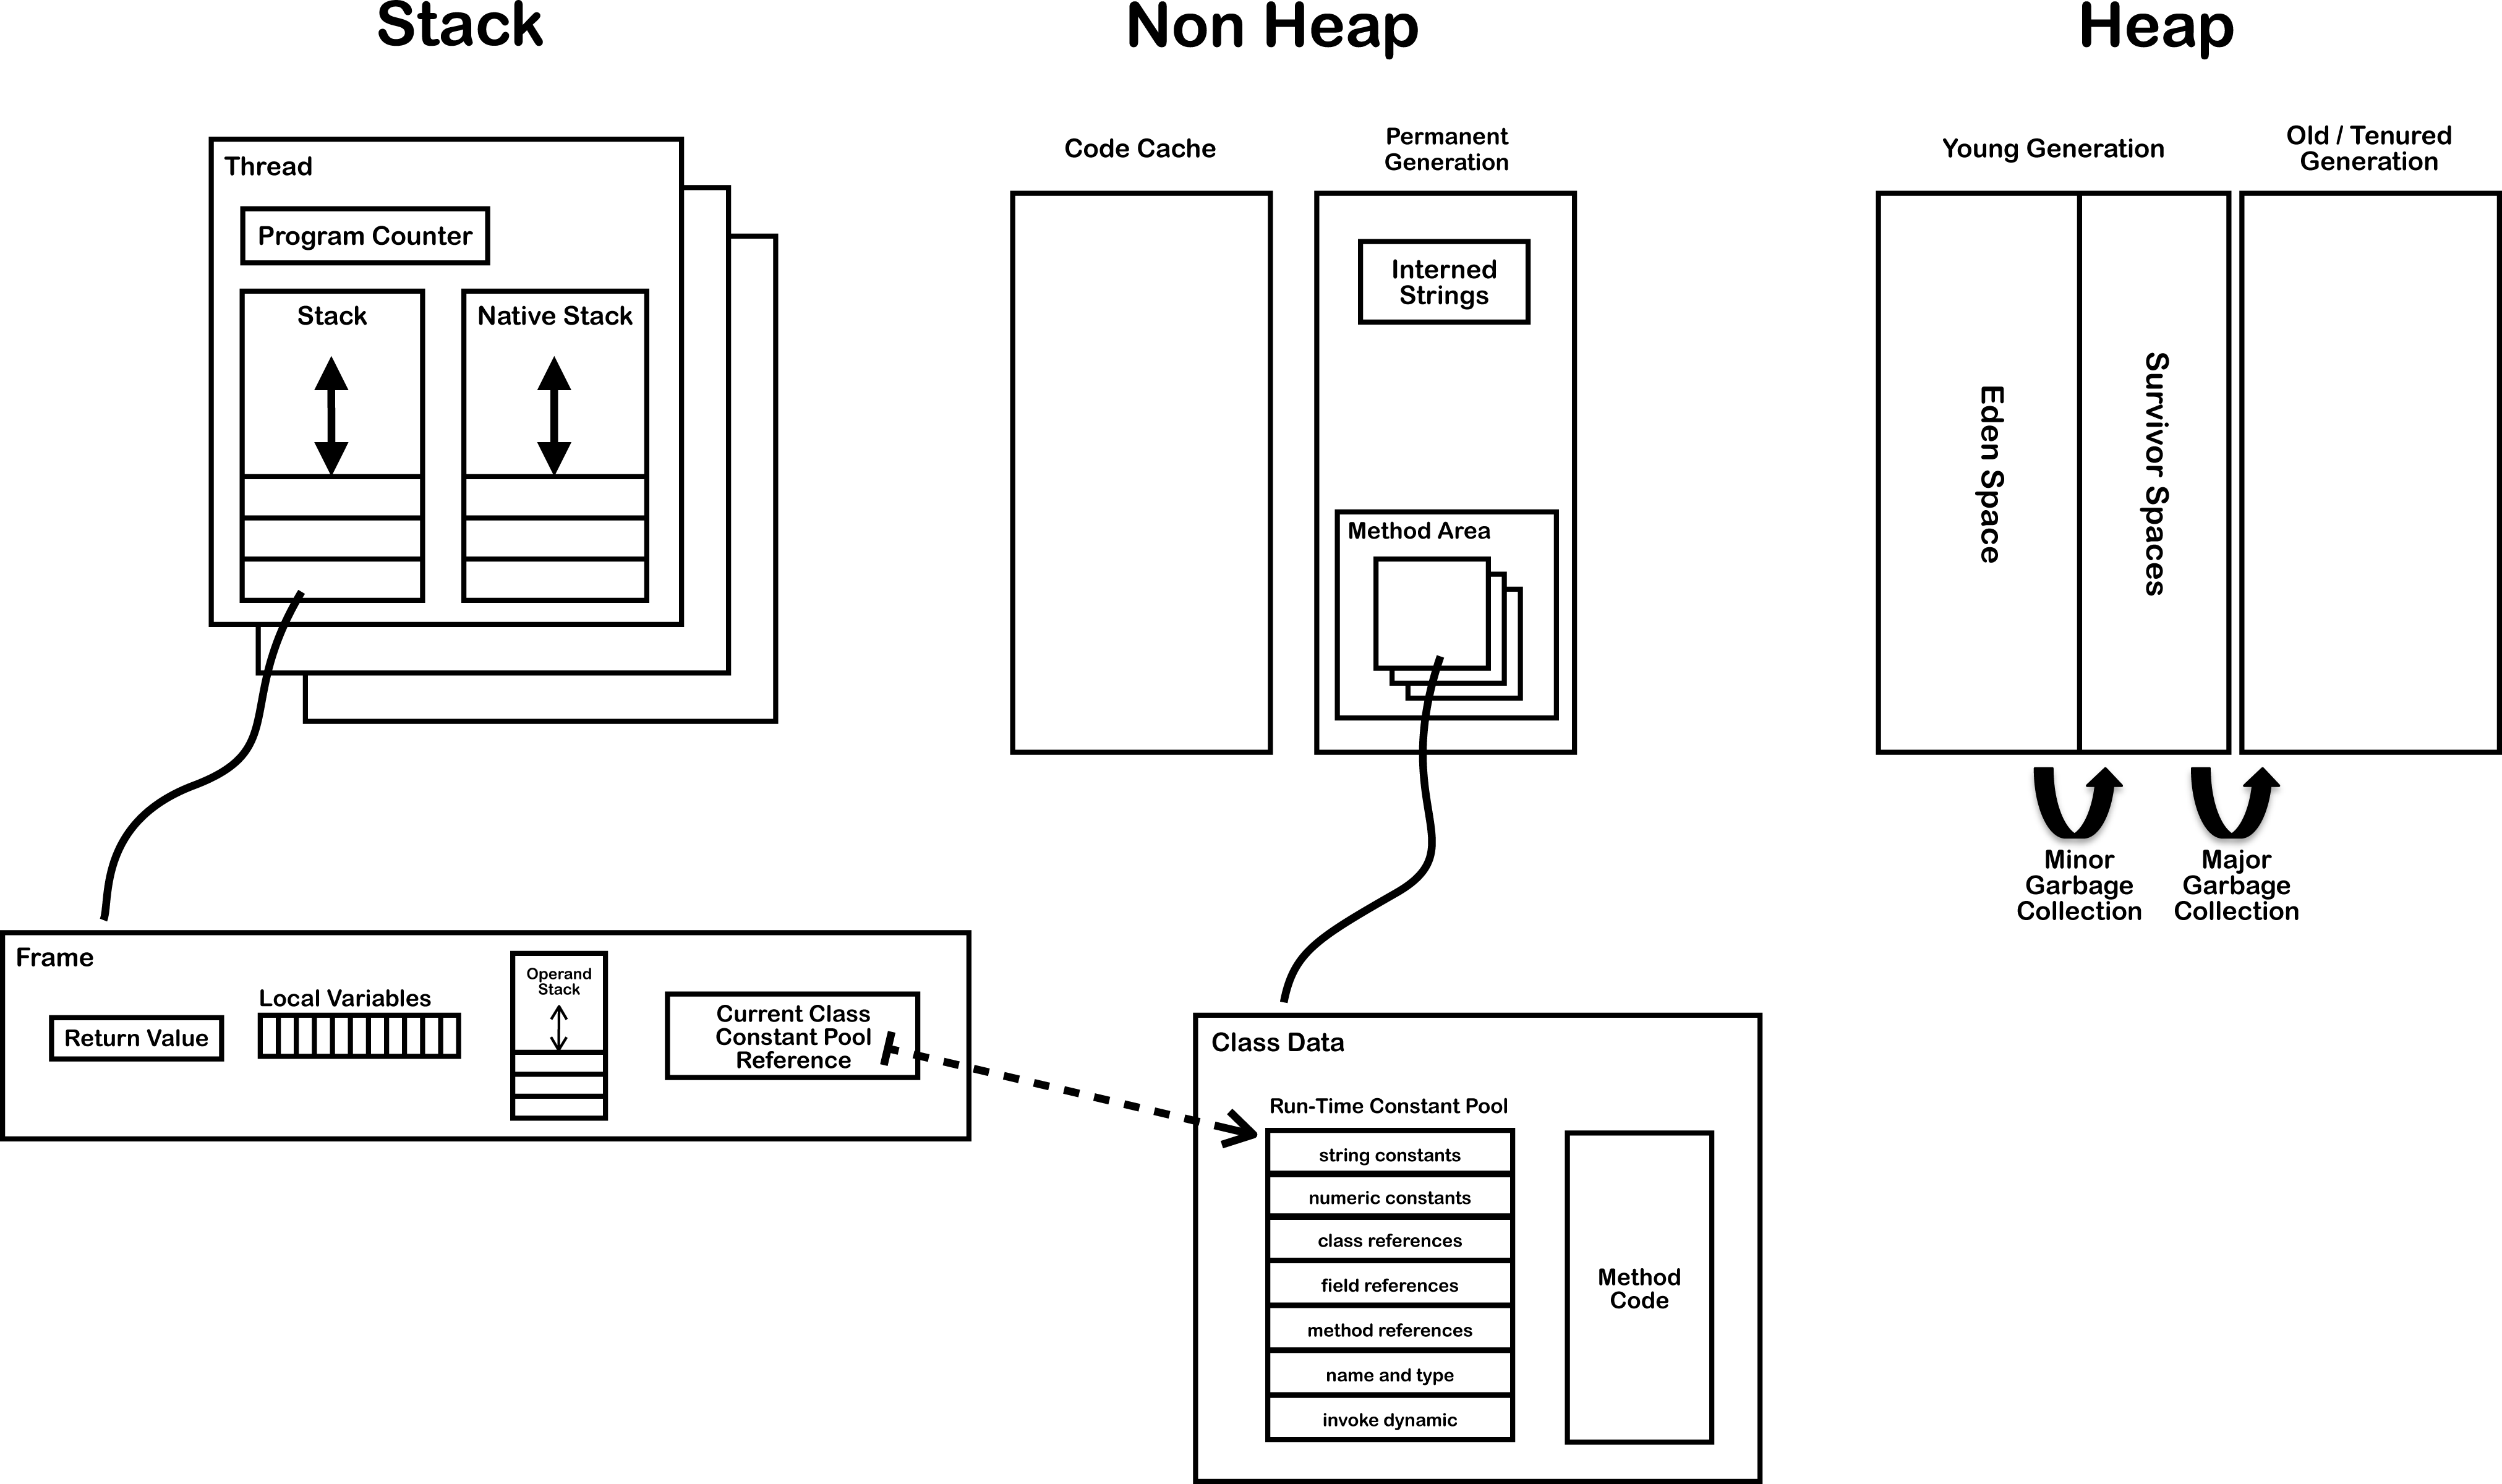
\includegraphics[width=\textwidth]{picturedir/JVMInternalArchitecture.png}\\
  \caption{JVM Internal Architecture - 1}\label{fig:jvm}
\end{figure}

\begin{figure}
  \centering
  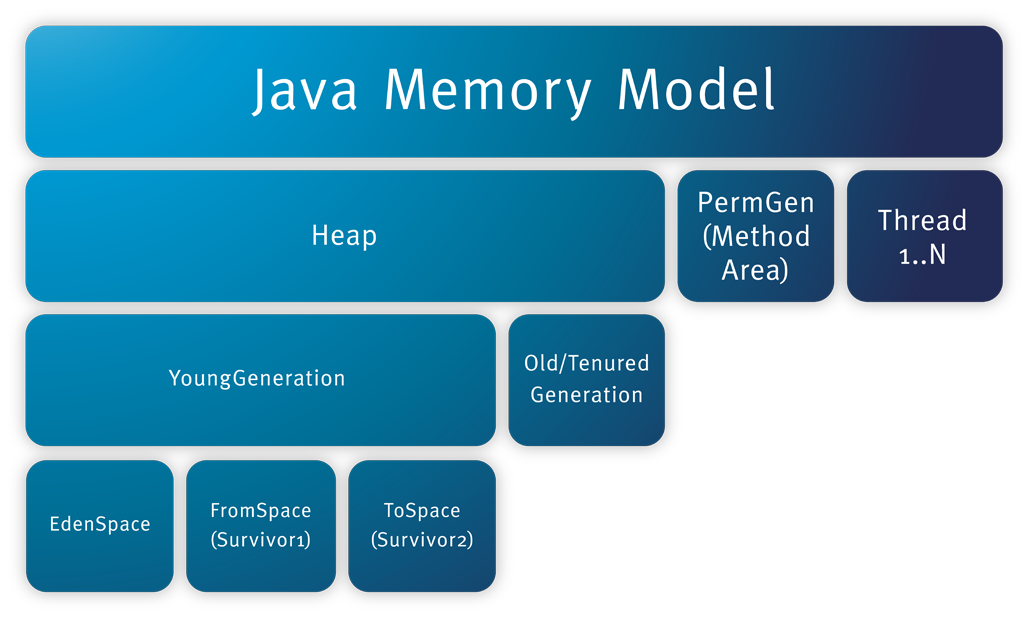
\includegraphics[width=\textwidth]{picturedir/JVMRuntimeDataArea.png}\\
  \caption{JVM Internal Architecture - 2}\label{fig:jvm2}
\end{figure}

\section[What is JVM]{什么是JVM}
Java Virtural Machine(JVM)可能有三种解释:
\begin{enumerate}
  \item The abstract specification,即JVM规范
  \item A concrete implementation,即一个具体的JVM实现
  \item A runtime instance,即一个运行时JVM实例
\end{enumerate}
简单一点儿理解,Java Virtual Machine可能指的是"specification"、"implementation"、
"instance"。

\section[Lifetime of JVM instance]{Lifetime of JVM instance}
JVM instance的使命就是“运行Java application”,Java application启动时创建,结束时
销毁。Java application和JVM instance是一一对应的,即每个Java application都运行在
一个“单独”的JVM instance中,如果一个电脑上同时运行了3个Java application,那么将会有
3个JVM instance同时存在。

运行时内存布局大致如下:
\begin{verbatim}
0GB            约1GB                 | <------Xmz----> 4GB
| OS & C-runtime | JVM | Native heap |   Java heap(s)   |
\end{verbatim}

\section[class file format]{class file format}
这一节的内容来自\href{http://hxraid.iteye.com/blog/687660}{这个}网页和JVM Spec 8。

\subsection[整体布局]{整体布局}
class文件整体布局如图\ref{fig:dotclass}所示,具体数据结构如下(来自JVM Spec 8),

\begin{figure}
  \centering
  % Requires \usepackage{graphicx}
  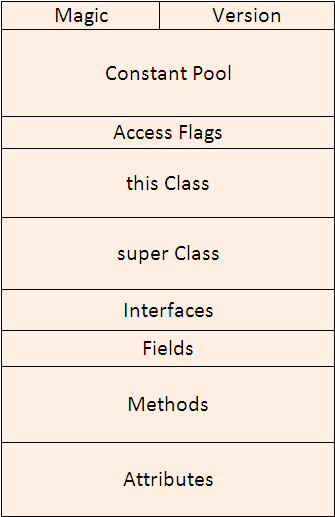
\includegraphics[width=.4\textwidth]{picturedir/JavaClassFileLayout.png}\\
  \caption{.class文件布局}\label{fig:dotclass}
\end{figure}

\begin{javacode}
ClassFile {
  u4 magic;
  u2 minor_version;
  u2 major_version;
  u2 constant_pool_count;
  cp_info constant_pool[constant_pool_count-1];
  u2 access_flags;
  u2 this_class;
  u2 super_class;
  u2 interfaces_count;
  u2 interfaces[interfaces_count];
  u2 fields_count;
  field_info fields[fields_count];
  u2 methods_count;
  method_info methods[methods_count];
  u2 attributes_count;
  attribute_info attributes[attributes_count];
}
\end{javacode}

进一步,各种info数据结构,

\begin{javacode}
cp_info {
  u1 tag;
  u1 info[];
}

field_info {
  u2 access_flags;
  u2 name_index;
  u2 descriptor_index;
  u2 attributes_count;
  attribute_info attributes[attributes_count];
}

method_info {
  u2 access_flags;
  u2 name_index;
  u2 descriptor_index;
  u2 attributes_count;
  attribute_info attributes[attributes_count];
}

attribute_info {
  u2 attribute_name_index;
  u4 attribute_length;
  u1 info[attribute_length];
}
\end{javacode}

class文件由8比特的字节流组成,全部字节流构成15个有意义的条目。
\begin{enumerate}
  \item magic number,0xCAFEBABE,表明一个文件是.class文件
  \item minor version, major version,主次版本号
  \item constant pool count,常量池大小
  \item constant pool,大小不固定,常量池,详见\ref{sec:constantpool}节
  \item access flag,表明类/接口、访问修饰符、是否抽象类、是否final类
  \item this class,它是一个常量池索引
  \item super class,它是一个常量池索引
  \item interface count, interface,接口数量以及接口的具体信息
  \item fields count, fields,属性的数量及其具体信息
  \item method count, methods,方法的数量及其具体信息(包括方法的实现)
\end{enumerate}

\subsection[常量池]{常量池}
\label{sec:constantpool}
常量池是由一个个item组成,就像一个表格,所有item总共有如下不同的类型,
每一种类型都由一个tag(1字节的常数)来标识,各种不同类型的数据结构定义
如下(来自JVM Spec 8,另外还有几种增加的类型没有列出),

\begin{javacode}
// 除了基本类型和UTF8类型存在“实际”数据以外,其他都是保存index而已!
CONSTANT_Class_info {
  u1 tag;
  u2 name_index;
}
CONSTANT_Fieldref_info {
  u1 tag;
  u2 class_index;
  u2 name_and_type_index;
}
CONSTANT_Methodref_info {
  u1 tag;
  u2 class_index;
  u2 name_and_type_index;
}
CONSTANT_InterfaceMethodref_info {
  u1 tag;
  u2 class_index;
  u2 name_and_type_index;
}
CONSTANT_String_info {
  u1 tag;
  u2 string_index;
}
CONSTANT_Integer_info {
  u1 tag;
  u4 bytes; // int占4个字节
}
CONSTANT_Float_info {
  u1 tag;
  u4 bytes; // float占4个字节
}
CONSTANT_Long_info {
  u1 tag;
  u4 high_bytes; // long占8个字节
  u4 low_bytes;
}
CONSTANT_Double_info {
  u1 tag;
  u4 high_bytes; // double占8个字节
  u4 low_bytes;
}
CONSTANT_NameAndType_info {
  u1 tag;
  u2 name_index;
  u2 descriptor_index;
}
CONSTANT_Utf8_info {
  u1 tag;
  u2 length;
  u1 bytes[length]; // 所有的“符号”都以UTF8形式存在
}
\end{javacode}

这些类型的tag值如表\ref{tab:constantpooltype}所示。

\begin{table}
\centering
\begin{tabular}{r|c|l}
Type & Flag\newline(1 byte) & Format \\
\hline\hline
CONSTANT\_Utf8 & 1 & <flag> <length> <data>\\
CONSTANT\_Integer & 3 & <flag> <data>\\
CONSTANT\_Float & 4 & <flag> <data>\\
CONSTANT\_Long & 5 & <flag> <data>\\
CONSTANT\_Double & 6 & <flag> <data>\\
CONSTANT\_Class & 7 & <flag> <index>\\
CONSTANT\_String & 8 & <flag> <index>\\
CONSTANT\_Fieldref & 9 & <flag> <index>\\
CONSTANT\_Methodref & 10 & <flag> <index>\\
CONSTANT\_InterfaceMethodref & 11 & <flag> <index>\\
CONSTANT\_NameAndType & 12 & <flag> <index>\\
\hline
\end{tabular}
\caption{Constant Pool format}\label{tab:constantpooltype}
\end{table}

需要注意的是真正数据存在于各种基本类型以及UTF8类型中,
其他的索引最终都要落到某个UTF8的数据处,这些数据即为
“符号”,如类的全限定名称,方法的完整签名等,运行时的
“符号解析”解析的就是这里的符号,其实就是一些字符串而已。

整体结构,

\begin{javacode}
/*
类文件 {
    0xCAFEBABE,
    小版本号,
    大版本号,
    常量池大小,
    常量池数组,
    访问控制标记,
    当前类信息,
    父类信息,
    实现的接口个数,
    实现的接口信息数组,
    域个数,
    域信息数组,
    方法个数,
    方法信息数组,
    属性个数,
    属性信息数组
}
*/
\end{javacode}

\subsection[实例解析]{实例解析}
以如下代码编译出来的class文件,逐个字节分析。

\begin{javacode}
package hr.test;
public class ClassTest {
  private int itemI = 0;
  private static String itemS = "我们";
  private final float PI = 3.1415926F;

  public ClassTest() { }

  public int getItemI() {
    return this.itemI;
  }

  public static String getItemS() {
    return itemS;
  }

  public static void main(String[] args) {
    ClassTest ct = new ClassTest();
  }
}
\end{javacode}

下面是逐字节分析,每个字节翻译为十进制数字。

%\input{srcdir/analyse.txt}

\begin{description}
\item[magic number:] 202 254 186 190
\item[minor version:] 0 0
\item[major version:] 0 50
\item[constant pool:] 0 43 常量池的长度,index从1开始,0被保留
	\begin{enumerate}
	\item 7 0 2\\
		对类ClassTest的符号引用(7为标志  02指向了常量池的索引2的位置)
	\item 1 0 17 104 114 47 116 101 115 116 47 67 108 97 115 115 84 101 115 116\\
		类全限定名"hr\bs test\bs ClassTest"
	\item 7 0 4\\
		对类Object的符号引用
	\item 1 0 16 106 97 118 97 47 108 97 110 103 47 79 98 106 101 99 116\\
		超类全限定名"java/lang/Object"
	\item 1 0 5 105 116 101 109 73\\
		第1个类字段名"itemI"
	\item 1 0 1 73\\
		第1个类字段类型为整型'I'
	\item 1 0 5 105 116 101 109 83\\
		第2个类字段名"itemS"
	\item 1 0 18 76 106 97 118 97 47 108 97 110 103 47 83 116 114 105 110 103 59\\
		第2个类字段类型的全限定名"Ljava/lang/String"
	\item 1 0 2 80 73\\
		第3个类字段名"PI"
	\item 1 0 1 70\\
		第3个类字段类型为'F'
	\item 1 0 13 67 111 110 115 116 97 110 116 86 97 108 117 101\\
		第3个类字段为常量"ConstantValue"
	\item 4 64 73 15 218\\
		第3个类字段float字面值,占4bytes(3.1415926)
	\item 1 0 8 60 99 108 105 110 105 116 62\\
		初始化方法名"<clinit>"
	\item 1 0 3 40 41 86\\
		方法的返回类型为"()V",即void
	\item 1 0 4 67 111 100 101\\
		"Code"
	\item 8 0 17\\
		String字符串字面值(0 17表示索引17)
	\item 1 0 6 230 136 145 228 187 172\\
		"我们"
	\item 9 0 1 0 19\\
		指向第2个字段的引用(0 1指向索引1,0 19指向索引19)
	\item 12 0 7 0 8\\
		指向第2个字段的名字和描述符的索引,
	\item 1 0 15 76 105 110 101 78 117 109 98 101 114 84 97 98 108 101\\
		"LineNumberTable"
	\item 0 18 76 111 99 97 108 86 97 114 105 97 98 108 101 84 97 98 108 101\\
		"LocalVariableTable"
	\item 1 0 6 60 105 110 105 116 62\\
		表示初始化方法名"<init>"
	\item 10 0 3 0 24\\
		指向父类Object的构造器方法,0 3表示父类名常量表的索引,0 24表示存放该方法名称和描述符的引用的常量表的索引
	\item 12 0 22 0 14\\
		指向方法名和描述符的常量表的索引。0 22是方法名的常量表索引,0 14是描述符的常量表索引
	\item 9 0 1 0 26\\
		指向第1个字段的引用, 0 1表示字段所属类型的索引,0 26表示字段名和描述符的索引
	\item 12 0 5 0 6\\
		指向第1个字段的名字和描述符的索引
	\item 9 0 1 0 28\\
		指向第3个字段的引用, 0 1表示字段所属类型的索引,0 28表示字段名和描述符的索引
	\item 12 0 9 0 10\\
		指向第3个字段的名字和描述符的索引
	\item 1 0 4 116 104 105 115\\
		隐含参数符号"this"
	\item 1 0 11 76 67 108 97 115 115 84 101 115 116 59\\
		"LClassTest;"
	\item 1 0 8 103 101 116 73 116 101 109 73\\
		方法名"getItemI"
	\item 1 0 3 40 41 73\\
		方法描述符"()I",即返回类型为int
	\item 1 0 8 103 101 116 73 116 101 109 83\\
		方法名"getItemS"
	\item 1 0 20 40 41 76 106 97 118 97 47 108 97 110 103 47 83 116 114 105 110 103 59\\
		方法描述符"()Ljava/lang/String;"
	\item 1 0 4 109 97 105 110\\
		主方法名"main"
	\item 1 0 22 40 91 76 106 97 118 97 47 108 97 110 103 47 83 116 114 105 110 103 59 41 86\\
		主方法中的参数的字符串数组类型名"()Ljava/lang/String;)V"
	\item 10 0 1 0 24\\
		指向当前 ClassTest 类的构造器方法,0 1表示存放当前类名的常量表的索引。0 24是存放方法名和描述符的符号引用的常量表索引。
	\item 1 0 4 97 114 103 115\\
		参数"args"
	\item 1 0 19 91 76 106 97 118 97 47 108 97 110 103 47 83 116 114 105 110 103 59\\
		字符串数组"[Ljava/lang/String;"
	\item 1 0 2 99 116\\
		对象符号"ct"
	\item 1 0 10 83 111 117 114 99 101 70 105 108 101\\
		"SourceFile"
	\item 1 0 14 67 108 97 115 115 84 101 115 116 46 106 97 118 97\\
		"ClassTest.java"
	\end{enumerate}
\item [access flags:] 0 33 访问标志:public
\item [this Class:] 0 1 指向当前类的符号引用在常量池中的索引
\item [super Class:] 0 3 指向当前类的父类的符号引用在常量池中的索引
\item [inteface count:] 0 0 接口的数量
\item [field count:] 0 3 字段的数量
\item [fields:] fields的具体内容
	\begin{enumerate}
	\item 字段 itemI\\
		0 2  --- private 修饰符\\
		0 5  --- 字段名在常量池中的索引,字段itemI\\
		0 6  --- 字段的描述符(所属类型)在常量池中的索引\\
		0 0  --- 字段的属性信息表(attribute\_info)的数量
	\item 字段 itemS\\
		0 10 ---- private static 修饰符\\
		0 7  --- 字段名在常量池中的索引,字段itemS\\
		0 8  --- 字段的描述符(所属类型)在常量池中的索引\\
		0 0  --- 字段的属性信息表(attribute\_info)的数量
	\item 字段 PI\\
		0 18 --- private final 修饰符\\
		0 9  --- 字段名在常量池中的索引,//字段PI\\
		0 10 --- 字段的描述符(所属类型)在常量池中的索引\\
		0 1  --- 字段的属性信息表(attribute\_info)的数量\\
		0 11 --- 属性名在常量池中的索引。即ConstantValue\\
		0 0 0 2 --- 属性所占的字节长度\\
		0 12 --- 属性值在常量池中的索引。即常量字面值
	\end{enumerate}
\item [method count:] 0 5 方法的数量
\item [methods:] methods的内容
	\begin{enumerate}
	\item 类的静态数据初始化方法<clinit>\\
		0 8  --- static 修饰符(所有的初始化方法都是static的)\\
		0 13 --- 在常量池中的索引。初始化方法名<clinit>,该方法直接由JVM在特定的时候调用,并非由字节码生成。\\
		0 14 --- 在常量池中的索引。返回类型为void。\\
		0 1  --- 属性数量\\
		0 15 --- 属性名 在常量池中的索引。即code\\
		0 0 0 42 ---  属性所占的字节长度42\\
		0 1 0 0 0 0 0 6 18 16 179 0 18 177 0 0 0 2 0 20 0 0 0 10 0 2 0 0 0 5 0 5 0 2 0 21 0 0 0 2 0 0 --- 该方法的字节码指令序列和其他信息
	\item 类的普通实例数据的初始化方法,针对类构造器生成的<init>方法。\\
		0 1  --- public 修饰符\\
		0 22 --- 构初始化方法名<init>\\
		0 14 --- 构造器的返回类型为void\\
		0 1  --- 属性数量\\
		0 15 ---  属性名在常量池中的索引。即Code\\
		0 0 0 70 -- 属性所占的字节长度70\\
		0 2 0 1 0 0 0 16 42 183 0 23 42 3 181 0 25 42 18 12 181 0 27 177 0 0 0 2 0 200 0 0 18 0 4 0 0 0 8 0 4 0 4 0 9 0 6 0 15 0 9 0 21 0 0 0 12 0 10 0 0 16 0 29 0 30 0 0
		---	该方法的字节码指令序列和其他信息
	\item getItemI方法\\
		0 1  --- public 修饰符\\
		0 31 --- 在常量池中的索引。方法名getItemI\\
		0 32 --- 在常量池中的索引。方法返回类型为int\\
		0 1  --- 属性数量\\
		0 15 --- 属性名在常量池中的索引。即Code\\
		0 0 0 47 ---  属性所占的字节长度70\\
		0 1 0 1 0 0 0 5 42 180 0 25 172 0 0 0 2 0 20 0 0 0 6 0 1 0 0 0 12 0 21 0 0 0 12 0 1 0 0 0 5 0 29 0 30 0 0 --- 该方法的字节码指令序列和其他信息
	\item getItemS方法\\
		0 9  --- public static 修饰符\\
		0 33 --- 在常量池中的索引。方法名getItemS\\
		0 34 --- 在常量池中的索引。方法返回类型为String\\
		0 1  --- 属性数量\\
		0 15 --- 属性名在常量池中的索引。即Code\\
		0 0 0 36 ---  属性所占的字节长度36\\
		0 1 0 0 0 0 0 4 178 0 18 176 0 0 0 2 0 20 0 0 0 6 0 1 0 0 0 16 0 21 0 0 0 2 0 0 --- 该方法的字节码指令序列和其他信息
	\item main方法\\
		0 9  --- public static 修饰符\\
		0 35 ---  在常量池中的索引。主方法名main\\
		0 36 --- 在常量池中的索引。方法返回类型为String[]\\
		0 1  --- 属性数量\\
		0 15 ---  属性名在常量池中的索引。即Code\\
		0 0 0 65 --- 属性所占的字节长度36\\
		0 2 0 2 0 0 0 9 187 0 1 89 183 0 37 76 177 0 0 0 2 0 20 0 0 0 10 0 2 0 0 0 20 0 8 0 21 0 21 0 0 0 22 0 2 0 0 0 9 0 38 0 39 0 0 0 8 0 1 0 40 0 30 0 1 0 1 0 41 0 0 0 2 0 42
		--- 该方法的字节码指令序列和其他信息
	\end{enumerate}
\end{description}


\section[Rumtime object in memory]{运行时数据模型}
本节\href{http://www.programcreek.com/2011/11/what-do-java-objects-look-like-in-memory/}{参考网址}。

\subsection[Fields in memory]{Fields in memory}
运行时期,对象在内存中的样子大致如图\ref{fig:base}所示。
\begin{figure}
  \centering
  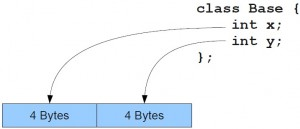
\includegraphics[width=0.8\textwidth]{picturedir/base.jpg}\\
  \caption{Runtime object in Heap}\label{fig:base}
\end{figure}

存在继承关系时的情形如图\ref{fig:derived}所示。
\begin{figure}
  \centering
  % Requires \usepackage{graphicx}
  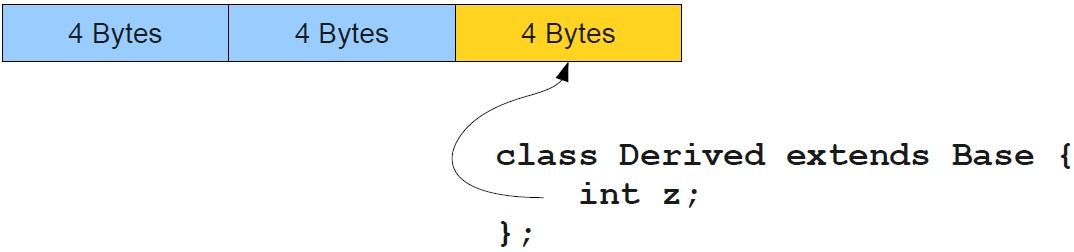
\includegraphics[width=0.8\textwidth]{picturedir/derived.jpg}\\
  \caption{Objects of Hierachy in Heap}\label{fig:derived}
\end{figure}

\subsection[Methods in memory]{Methods in memory}
类似于属性在内存中的布局,方法也可以同样布局,如图\ref{fig:novtable}所示。
\begin{figure}
  \centering
  % Requires \usepackage{graphicx}
  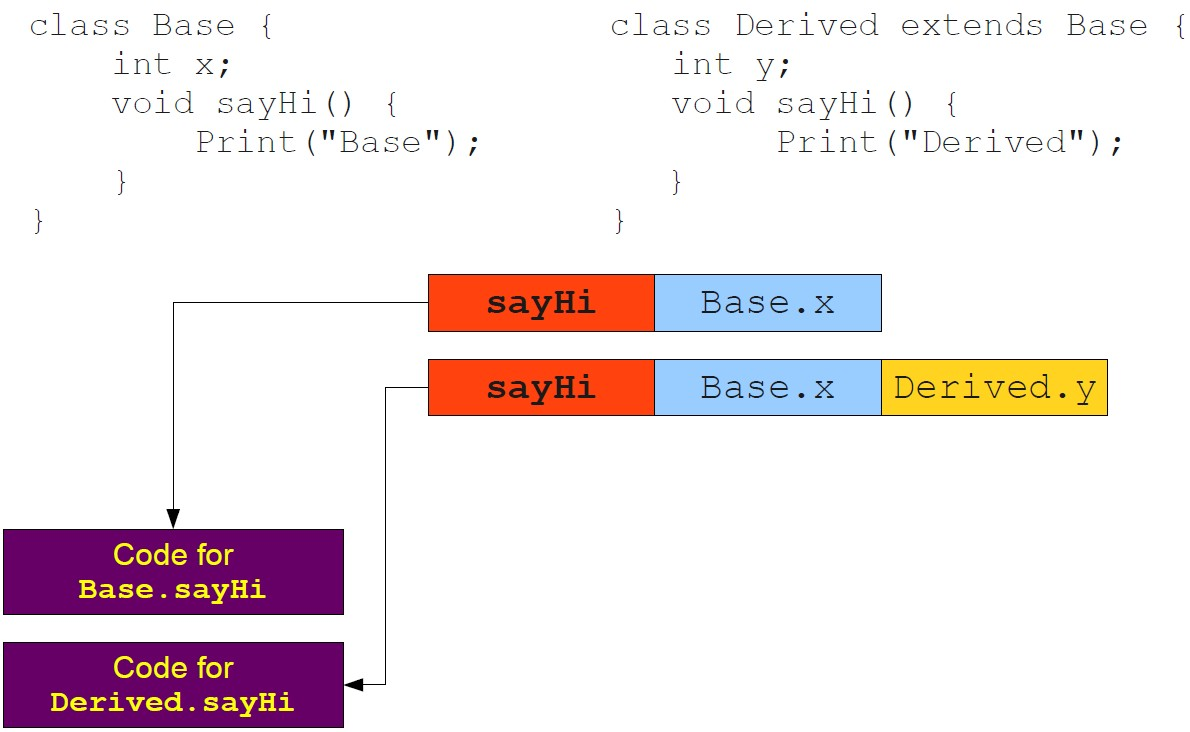
\includegraphics[width=0.8\textwidth]{picturedir/functions-without-vtable.jpg}\\
  \caption{Objects in Heap without VTable}\label{fig:novtable}
\end{figure}
可是,这样一来每个对象都有一堆重复的method pointer,占空大,效率低,不划算,
改进一下,每个类增加一个函数表,而每个对象只需一个指向该函数表的指针即可,
如图\ref{fig:vtable}所示,注意父类、子类有覆盖(override)关系的函数在函数表中
的位置必须是一样的,详见第\ref{sec:dynamicbinding}节。
\begin{figure}
  \centering
  % Requires \usepackage{graphicx}
  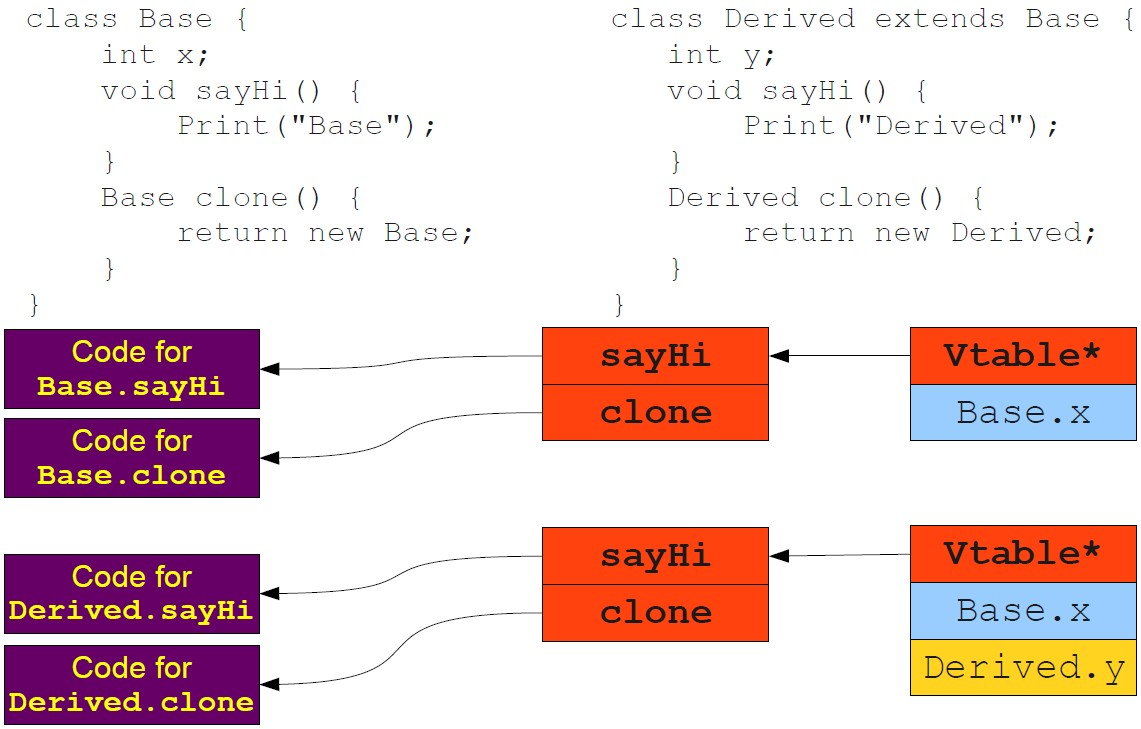
\includegraphics[width=.8\textwidth]{picturedir/objects-in-memory-optimization.jpg}\\
  \caption{Object layout with VTable}\label{fig:vtable}
\end{figure}


\section[static-binding vs dynamic binding]{static-binding vs dynamic binding}
\label{sec:dynamicbinding}

\section[class loader]{class loader}
Java的class loader分为两种:
\begin{enumerate}
  \item built-in class loader: 内置的类加载器只有一个,叫做bootstrap class loader
    \begin{itemize}
      \item Bootstrap: 加载[JRE]\bs lib\bs rt.jar和-Xbootclasspath指定的目录
    \end{itemize}
  \item user-defined class loader: JDK中预先提供两个用户自定义类加载器:
    \begin{itemize}
      \item ExtClassLoader: 加载[JRE]\bs lib\bs ext\*.jar和-Djava.ext.dirs指定的目录
      \item AppClassLoader: CLASSPATH环境变量和-Djava.class.path指定的目录
    \end{itemize}
\end{enumerate}
Bootstrap内置于JVM实现,由C++部分实现,所以没有Java Class对象与之对应(null与之对应),
用户自定义的类加载器都有Java层Class对象与之对应。Java提供ClassLoader类,所有用户自定义的
加载器都继承自该类,如图\ref{fig:classloadertree}所示。
% class inheret tree
\begin{figure}
  \centering
  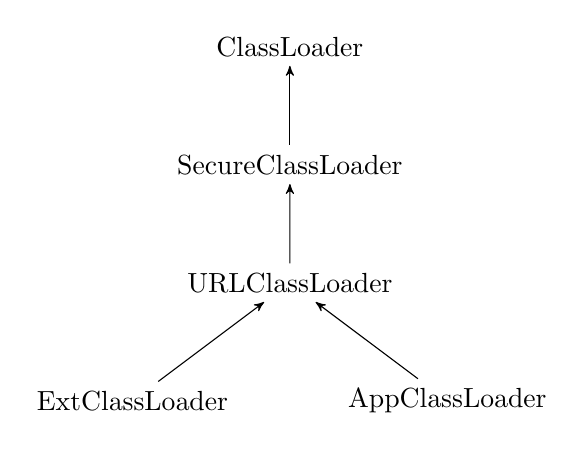
\begin{tikzpicture}[<-,>=stealth',level/.style={sibling distance = 4cm,level distance=1.5cm}]
  \node {ClassLoader}
  child {
    node {SecureClassLoader}
    child {
      node {URLClassLoader}
      child {
        node {ExtClassLoader}
      }
      child {
        node {AppClassLoader}
      }
    }
  };
  \end{tikzpicture}
  \caption{JDK中自定义类的(OOP)继承体系}\label{fig:classloadertree}
\end{figure}

\subsection[DIY class loader]{DIY class loader}
自定义class loader只需继承ClassLoader类即可,该类中设计到自定义类加载器的有
如下这些方法:\\
\begin{javacode}
public Class<?> loadClass(String name)
  throws ClassNotFoundException { }
protected Class<?> findClass(String name)
  throws ClassNotFoundException { }
protected final Class<?> defineClass(String name, byte[] b, int off, int len,
  ProtectionDomain protectionDomain) throws ClassFormatError { }

protected synchronized Class<?> loadClass(String name, boolen resolve)
  throws ClassNotFoundException { }
public final ClassLoader getParent(){ }
protected final Class<?> findLoadedClass(String name) { }
protected final void resolveClass(Class<?> c) { }
\end{javacode}

其中,loadClass()会实现代理模式,详见第\ref{sec:delegationmodel}节,
所以不要轻易override这个方法,自定义class loader时只需override findClass(),
标准的做法是这样的:\\
\begin{javacode}
class MyClassLoader extends ClassLoader {

  public Class findClass(String name) {
    byte[] b = loadClassData(name);
    return defineClass(name, b, 0, b.length);
  }

  private byte[] loadClassData(String name) {
    // load the class data from file system, network etc.
  }
}
\end{javacode}

下面是一个完整的例子,

\begin{javacode}
class MyClassLoader extends ClassLoader {
  private static String prefix = "path/to/project/";

  public MyClassLoader() { // 使用AppClassLoader作为其parent
    super();
  }
  public MyClassLoader(ClassLoader parent) {
    super(parent); // if parrent == null then use bootstrap class loader as parent
  }

  @Override
  public Class findClass(String name) throws ClassNotFoundException {
    System.out.println("can not load class, not try finding: " + name);
    byte[] data = null;
    try {
      data = getClassData(name);
    } catch (IOException e) {
      e.printStackTrace();
    }
    return defineClass(name, data, 0, data.length);
  }

  private byte[] getClassData(String name) throws IOException {
    File f = new File(prefix + convertPath(name) + ".class");
    FileInputStream input = new FileInputStream(f);
    byte[] data = new byte[(int) f.length()];
    input.read(data);
    input.close();
    return data;
  }

  private String convertPath(String dotPath) {
    StringBuilder builder = new StringBuilder();
    for(String s : dotPath.split("\\.")) {
      builder.append(s + "/");
    }
    return builder.subSequence(0, builder.length()-1).toString();
  }
}
// test
void testClassLoader() {
  MyClassLoader loader1 = new MyClassLoader(); // use AppClassLoader as parent
  Class c1 = loader1.loadClass("com.example.javademo.ThisSuper");
  ThisSuper o1 = (ThisSuper) c1.newInstance();

  MyClassLoader loader2 = new MyClassLoader(null); // use Bootstrap as parent
  Class c2 = loader2.loadClass("com.example.javademo.ThisSuper");

  System.out.println(c1 == c2); // false
}
\end{javacode}

\subsection[parent delegation model]{parent delegation model}
\label{sec:delegationmodel}
Java管理这些类加载器时采用delegation model(代理模式),每个loader都有一个parent属性
(定义在ClassLoader类中),load class时首先使用parent进行加载,如果无法加载再自行加载,

\begin{javacode}
// implementation of loadClass() in ClassLoader
...
// First, check if the class has already been loaded
Class c = findLoadedClass(name);
if (c == null) {
  try {
    // Second, try to delegate class-loading to 'parent'
    if (parent != null) {
      c = parent.loadClass(name, false);
    } else {
      c = findBootstrapClass0(name);
    }
  } catch (ClassNotFoundException e) {
    // finally, find class using findClass()
    c = findClass(name);
  }
}
...
\end{javacode}

注意,这是个递归调用,最终的结果就是从child到parent进行扫描,如果没有找到class,
就再从parent到child依次调用findClass(),这是一个从child到parent然后再返回到child
的过程,中间任何一步找到class就结束整个流程。

为何要搞一个代理模式处理呢?为了安全!

代理模式可以保证优先从Java Core API中加载类,如java.lang.String类,走到Bootstrap
的时候已经找到了,所以即使用户自己重新定义String类,也不会被用到,这就保证了
核心库不被恶意替换掉。

但是,如果重写loadClass()函数的话就可能破坏代理模式,如Tomcat中的class loader
加载类的顺序正好跟这里的代理模式相反,不过在defineClass()的时候会有package检查,
如java.*这样的package是无法通过defineClass()重新定义的,而defineClass()是final的,
这就保证了核心库的安全性,除非用户不使用defineClass()而自己搞一套类定义机制出来
(可能吗?)。

\subsection[namespace]{namespace}
任何一个class都是由某一个class loader加载到JVM中的,在JVM中,一个类的唯一性并不
仅仅是靠package来保证,而是package和class loader一同保证,即不同class loader
完全可能加载同一个class到JVM,形成两个不同的class对象,这种机制就叫做namespace。

那么namespace是如何构成的呢?一个class loader构成一个namespace吗?No,这会造成
重复加载,想象一下一个class loader中就有一个String类,太浪费了!

答案是利用delegation model构成namespace,在HotSpot中,没加载一个类JVM内部都会
把它缓存起来,JVM内部维护一个巨大的哈希表:

$hash\;table: classname+loader \stackrel{hash}{\longrightarrow} class\;object$

加上代理模式,每个child loader都可以看到parent加载的class object,于是一个
class loader所能加载的class连同其parent所能加载的class就构成了一个namespace,
不同namespace之间无法相互访问,就像无法访问object(in heap)的private field一样。


\end{document}
